\documentclass{article}

\usepackage[xetex, colorlinks=true]{hyperref}
\usepackage[
   backend=biber,
   bibencoding=utf8,
   style=alphabetic,
   hyperref=true,
   % citestyle=authoryear-comp,
   backref=false,
   sortlocale=en,
   url=true,
   doi=false,
   eprint=false
 ]{biblatex}
\addbibresource{biblio.bib}

\newcommand\Coq{Coq}
\newcommand\R{R}
\newcommand\Cn{C}

\usepackage{minted}
\setminted{encoding=utf8}

\usepackage{tikz}
\usetikzlibrary{positioning}

\tikzset{
	box/.style = {
		draw = black,
        fill = white,
		rectangle,
		rounded corners = 2pt,
		text centered,
		minimum height = 5mm,
		minimum width = 10mm
	}
}

\title{Notes about \R}
\author{Martin Bodin}

\begin{document}

\maketitle

\section{Presentation of the Language}

\R{} is now a trending programming language for mathematicians.
In practise, it is presented as a read-eval-print-loop,
but it is also possible to write programs in it.
% The language enables easy integration of \Cn{} functions.
The language presents itself as a weakly typed programming language
manipulating different types of arrays.
The language is dynamic,
in the sense that most programs have a semantics.

\subsection{History}

\R{} is a programming language designed for statistics.
Its specification~\parencite{team2000r} is not precise:
in practise, it is specified by its main implementation~\parencite{Rwebsite}.

The original authors of \R{}~\parencite{ihaka1996r}
describe \R{} as a programming language similar to Scheme
which has been mutated to get a programming language similar to S.
In particular, \R{} features scoping and first-class functions
as Scheme.
Similarly to S, however, it is a lazy programming language.

It is a community driven programming language.
This means that most of what is used in a \R{} program comes from various libraries,
which can change the way the programming language behaves.
This can be compared with JavaScript,
and how libraries like jQuery changes the way programs look.

\subsection{Features}

\R{} is accompanied with a lot of features.
We detail here the ones relevant from the point of view
of it as a programming language.

\subsubsection{Promises}
\label{sec:promises}

The \R{} programming language is lazy.
This was a design choice:
it occurs often in \R{} to define a large array,
but then filter it to only consider a small number of cells.
Lazyness enables the programming language to focus on these cells
and only compute what is needed to display their content.

In practise, lazyness comes in the form of promises.
A promise is composed of a syntactic expression,
an environment, and an optional value.
If \R{} needs the result of promise,
it will check the optional value.
If it is present, the promise already has been computed
and the value is directly reused.
Otherwise, the promise’s expression is evaluated,
and the promise’s value is set to the returned value.
The evaluation of the expression might raises side effects.
%
A typical place where promises are defined
is during function calls.
\begin{minted}{R}
f <- function (x, y)
     if (x == 1) y
# “f” is now a function
f (1, 2 + 2) # The expression “2 + 2” becomes here a promise.
# The function “f” uses this promise, and it thus reduces to “4”.
f (1, a <- 1) # This promise has a side effect.
a # Returns 1. Note that the promise kept the initial environment:
  # Variable “a” has been defined in the initial environment.
f (0, b <- 1) # This promise has a side effect, but is not evaluated.
b # Returns an error.
\end{minted}

This lazyness feature of \R{} enables
language constructs like \mintinline{R}{if}
to be considered as \emph{functions}.
There are thus very few cases in the evaluation function
of \R{}, corresponding to the atomic types.
This also enables libraries to drastically change
the language’s syntax.

Function arguments can have default argument,
but in this case, it is still a promise.
In the following example,
Variable \mintinline{R}{y} is associated with
the promise \mintinline{R}{x} and the environment
created during the call (not the initial one).
But this environment may change during the function evaluation.
\begin{minted}{R}
x <- 1 # A global variable.
f <- function (x, y = x) { # Variable “y” receives the promise “x”.
       x <- 3 # We update Variable “x”.
       y      # Evaluates the promise.
       x <- 4 # We update again “x”.
       y      # The promise has already been evaluated.
     }
f (2) # The local variable “x” is set to 2.
# Returns 3.
\end{minted}

One of the goals of the \R{} programming language
is to enable easy graphical drawings,
through functions such as \mintinline{R}{plot}.
To express equations, \R{} uses promises.
Here is an example taken from the original paper~\parencite{ihaka1996r}.
\begin{minted}{R}
curve <- function (expr, from, to) {
           x <- seq (from, to, length = 500)
           y <- eval (substitute (expr))
           plot (x, y)
         }
\end{minted}
This function can then be invoked as
\mintinline{R}{curve (x^2 - 1, -2, 2)}
to draw the function \(f(x) = x^2 - 1\)
over the interval \([-2, 2]\).
Let us now understand what happens during
such a call.
First, Variable \mintinline{R}{expr}
is associated with he promise \mintinline{R}{x^2 - 1}
in the initial environment.
This may be seen strange as the initial environment
does not define any variable \mintinline{R}{x}.
Inside the scope of function \mintinline{R}{curve},
a variable \mintinline{R}{x} is defined, as a vector.
The function \mintinline{R}{substitute} is a special function,
as it manipulates the inner data type of the promise \mintinline{R}{expr}:
it replaces its inner environment with the current environment
(that is, the inner scope).
The variable \mintinline{R}{x} inside the promise
\mintinline{R}{expr} is now linked with the local
variable \mintinline{R}{x},
and the promise can be evaluated.


\subsubsection{Vectors}

In the previous example,
Variable \mintinline{R}{x} was associated the result
of \mintinline{R}{seq}, which is a numerical vector.
It can be surprising that we were able to compute
the expression \mintinline{R}{x^2 - 1},
as \mintinline{R}{x} is not a number.
The reason is that the operators \mintinline{R}{^} and \mintinline{R}{-}
applies on vectors, component by component.
The numbers \mintinline{R}{2} and \mintinline{R}{1}
in the expression are seen as vectors with only one component.
We cannot assign a variable with a number,
but we can assign it a numerical vector of size one,
and \R{} does it all the time.
As the vectors \mintinline{R}{2} and \mintinline{R}{1}
are not the same size than \mintinline{R}{x},
their values are reused in a cyclic manner.
In most cases, this is what the user wants,
but it can be surprising if the user thought that both
vectors had the same size but had not:
no warning will be emitted by \R{}.

One operation whose semantics can be difficult
to fully comprehend is the vector indexing.
Given a vector \mintinline{R}{v},
we can filter it by \mintinline{R}{v[i]}.
The behaviour of this operation will be very different,
depending on the nature of \mintinline{R}{i}.
\begin{itemize}
    \item If \mintinline{R}{i} is a logical vector\footnote{
          Logical vectors stores tri-valued booleans,
          which can be \mintinline{R}{TRUE}, \mintinline{R}{FALSE},
          or \mintinline{R}{NA} (not applicable).
          All base values have an \mintinline{R}{NA} value.
      }, then \mintinline{R}{i} is first repeated
      to match the size of \mintinline{R}{v}.
      Then, each index of \mintinline{R}{v} corresponding
      to the value \mintinline{R}{TRUE} from the index array \mintinline{R}{i}
      are conserved;
      each corresponding to \mintinline{R}{FALSE} are removed;
      and each corresponding to \mintinline{R}{NA} are replaced
      by the \mintinline{R}{NA} of the expected type.
    \item If \mintinline{R}{i} is a numerical vector,
      and that all its elements are positive, zero, or \mintinline{R}{NA},
      then the corresponding indexes of \mintinline{R}
      are taken in the given order, resulting in an array
      that can be thought of the same size than \mintinline{R}{i}.
      Indexes of \mintinline{R}{v} are however counted from
      \(1\), and all \(0\) in \mintinline{R}{i} are ignored.
      If \mintinline{R}{i} contains \mintinline{R}{NA},
      they yield \mintinline{R}{NA} in the resulting array.
      Values of \mintinline{R}{i} greater than the size of \mintinline{R}{v}
      results in \mintinline{R}{NA}.
      Note that a special case of this case is \mintinline{R}{v[1]},
      which returns an array with only one cell.
    \item If \mintinline{R}{i} is a non-empty numerical vector
      whose elements are all negative or zero,
      then the result is the array \mintinline{R}{v}
      in which all values whose index (starting from \(1\))
      is the opposite of a number in \mintinline{R}{i} are removed.
    \item If \mintinline{R}{i} is a vector of character strings,
      and that \mintinline{R}{v} is associated with a \mintinline{R}{names}
      attribute\footnote{
          Any \R{} object can be associated attributes.
          They are a simple name to value mapping,
          which can be updated at will.
      }.
      We do not detail this case in details,
      but \R{} then intuitively selects the cells of \mintinline{R}{v}
      by their names.
\end{itemize}

\subsubsection{Function Calls}

The part of \R{} source code dealing with function application,
and in particular in the part matching given argument to expected arguments,
is surprisingly long.
The reason is that there are several, separately simple, ways to call
a function.
Each of these ways then interoperate during the call,
making it quite complex.

We have seen in Section~\ref{sec:promises} that default arguments can be given
to a function argument:
if the argument is not provided, a promise is associated with the default value.
Arguments can also be given by name,
as in the \mintinline{R}{curve} example of the same section:
the function \mintinline{R}{seq} is given its argument named \mintinline{R}{length}
as a named argument,
overwriting the argument order.

Arguments can also be missing.
This does not break the function call.
However, if the associated promise is evaluated, then an error is thrown.
However, we can not provide more arguments than what a function expects,
resulting in an error during the function call.
It is however possible to provide a \mintinline{R}{...} formal argument
to a function definition.
When called, all additional arguments will be packed in a special array.

Surprisingly, named arguments are matched by prefix
(called “partial match” in \R{} source code) and not by exact name,
unless they are after a \mintinline{R}{...} formal argument.
For instance, in the example below,
we can refer to the argument \mintinline{R}{cd} as just \mintinline{R}{c}.
Exact matches have however higher priority to prefix:
although \mintinline{R}{ab} is a prefix of \mintinline{R}{abc},
as it exactly corresponds to the name of a formal argument,
\R{} do not mix them.
Also, exact matches are checked first, and partial matches second:
this is the reason why the call \mintinline{R}{f (ab = 2, a = 1, 3)}
below succeeds, assigning \mintinline{R}{abs} to \(1\).
\begin{minted}{R}
f <- function (abc, ab, cd) c(abc, ab, cd)
# All the expressions below returns the array 1 2 3.
f (1, 2, 3)
f (cd = 3, 1, 2)
f (c = 3, 1, 2)
f (ab = 2, 1, 2)
f (ab = 2, a = 1, 3)
f (a = 3, 1, 2) # Returns an error, as “a” is the prefix of several formal arguments.
\end{minted}


\section{\R{} Interpreters}

There are several variants of \R{} interpreters.

\subsection{The Main \R{} Interpreter}

\subsubsection{Concepts}
\label{sec:concepts}

Most \R{} objects are in the form of a \emph{basic language element}.
This is a \Cn{} structure composed of a tag and four pointers.
The tag precises the kind of the basic language element;
it can be for instance an integer vector, an environment, an expression, or an external pointer.
The meaning of the last three vectors depends on the flag.
%
For instance, for an environment, the first pointer is a pointer
to the current frame (associating each local variable to a value or a promise),
the second pointer points to the environment of the outer scope,
and the third pointer points to a hash (to enable faster checks).
%
For a list, the first pointer points to the first element of the list,
the second, to the rest of the list,
and the third, to an optional name for the first element.

\subsubsection{Main Files and Functions}
\label{sec:files}

This table shows the various main files of the \Cn{} source code of \R{}.

\begin{tabular}{|c|p{7cm}|}
    \hline
    \texttt{src/include/Internal.h} & Defines the basic language element structure. \\
    \hline
    \texttt{src/main/names.c} & Fills in the global environment, associating each \R{} construct/name to its corresponding \Cn{} function. \\
    \hline
    \texttt{src/main/eval.c} & Defines \Cn{} functions to evaluate expressions. In particular the function \mintinline{C}{eval}, taking an expression and an environment and evaluating the expression. \\
    \hline
    \texttt{src/main/match.c} & Contains various function to deal with the association between formal and given arguments in a function call. \\
    \hline
    \texttt{src/main/context.c} & Defines contexts, which is a structure used to manipulate informations relative to program points, for constructs like \mintinline{R}{break} or \mintinline{R}{return}. \\
    \hline
    \texttt{src/main/envir.c} & Defines various \Cn{} functions to manipulate environments. \\
    \hline
    \texttt{src/main/coerce.c} & Contains a \Cn{} functions to converts \R{} values to other types. It also contains the \mintinline{R}{substitute} function. \\
    \hline
\end{tabular}

These files change regularly,
but rarely in the \Cn{} part.
Most of the changes between the current (trunk) version
and in Version~\(3.0\) (from 2012, that is five years ago)
are changes in the preprocessor
(some architectures includes different headers),
added documentation in comments,
small type changes between similar types
(\mintinline{C}{unsigned long} updated to \mintinline{C}{size_t}),
code restructuration,
and more importantly,
new behaviours.
There new behaviours are mostly additional checks
and exceptions providing more behaviours
(or more precise behaviours) to the \R{} interpreter
for rare cases.

\subsection{FastR}

The \R{} runtime can be slow.
\cite{kalibera2014fast} propose a faster approach.


\section{Formalisation}

This section describes my approach to formalise \R{} in \Coq{}.

\subsection{Language Formalisation}

Following my experience with JSCert~\parencite{bodin2014trusted},
I think that it is important to have a specification
the closest possible to \R{} internals.
Indeed, JavaScript possesses structures in some way similar
to the basic language elements (see Section~\ref{sec:concepts}),
called completion triples.
In JSCert, we initially choose to represent these completion triples
as a \Coq{} inductive,
each case of the triples only containing the attributes that made sense for us.
For instance, a basic language element whose tag is “symbol”
will probably only use one pointer to represent the string of the symbol.
By we discovered later that a construct of JavaScript % The sequence
broke what we thought were invariants:
the standard manipulated the structure as is it was a \Cn{} structure,
breaking our type assumptions.
We were forced to start the formalisation again with a structure
closer to the standard.

I thus propose a formalisation based on the structure below.
Arrows represent trust relations,
those which are dashed are planned but not yet there.
It is inspired by the refinement methodology~\parencite{cohen2013refinements}:
produce several implementations,
one easier to specify and one easier (or more efficient) to implement,
then prove correct each one relatively to the next one.
\begin{center}
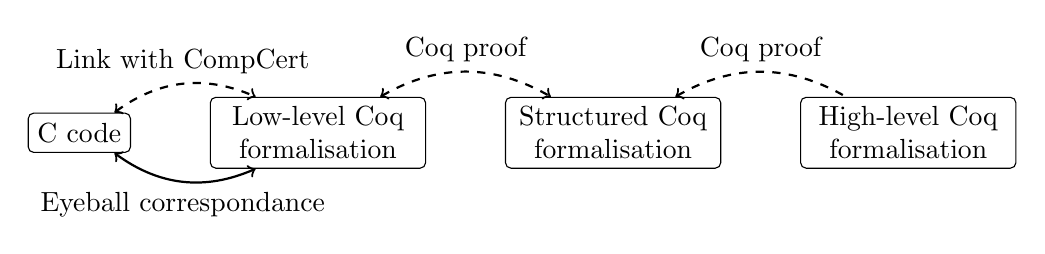
\begin{tikzpicture}
    \node [box] (C) {\Cn{} code} ;
    \node [box, right = 1cm of C] (low) {\parbox{25mm}{\centering{}Low-level \Coq{} formalisation}} ;
    \node [box, right = 1cm of low] (structured) {\parbox{25mm}{\centering{}Structured \Coq{} formalisation}} ;
    \node [box, right = 1cm of structured] (intuition) {\parbox{25mm}{\centering{}High-level \Coq{} formalisation}} ;

    \draw [<->, thick, dashed] (C) to [bend left] node [above] {Link with CompCert} (low) ;
    \draw [<->, thick] (low) to [bend left] node [below] {Eyeball correspondance} (C) ;
    \draw [<->, thick, dashed] (low) to [bend left] node [above] {\Coq{} proof} (structured) ;
    \draw [<-, thick, dashed] (structured) to [bend left] node [above] {\Coq{} proof} (intuition) ;
\end{tikzpicture}
\end{center}
At one end of the refinements is the \Cn{} source code of the \R{} interpreter.
As \R{} is defined by implementation,
this can be seen as a specification.
We in particular focus on the parts defining program evaluation
(mostly the files \texttt{src/include/Internal.h} and \texttt{src/main/eval.c}),
ignoring most constructs of the \R{} programming language.
A \Coq{} version of these \Cn{} definitions is defined,
with the aim to be the closest possible to the \Cn{} definition.
Some parts of the functions are dropped at this level,
such as error management.
At term, it is planned to use CompCert to prove that the \Coq{}
version is indeed identical to the chosen parts of the \Cn{} definition.

A structured \Coq{} formalisation is then defined.
This formalisation abstracts some low-level constructs,
such as pointers to basic language element
(which are heavily used in \R{}’s source code).
The expressions are also given a proper inductive at this stage,
although it is only weakly typed.
This inductive merely emphases with flag uses which pointers
of the basic language element structure.
It also makes explicit a subtlety of \Cn{} pointers,
which can be used for two distinct usages:
a pointer to one object,
or a pointer to an array of this object.
In this structured formalisation, the pointers to arrays
are replaced by a list,
which is much easier to manipulate in \Coq{}.

The last step of the process aims to fit
the intuition that the original had in mind when defining
the \R{} programming language~\parencite{ihaka1996r}.
Some advanced \R{} constructs may not fit such a high-level formalisation,
as they might break the underlying assumptions.


\subsection{What is Formalised}

The \Cn{} source code of \R{} is large.
It is thus out of the question to translate every \Cn{} function to \Coq{}.
I have focussed on the \mintinline{C}{eval} function from
\texttt{src/main/eval.c} and its dependencies.
This includes in particular the \Cn{} structures used to represent
\R{} expressions,
as well as a large parts of the files presented in Section~\ref{sec:files}.

\subsubsection{Structures}

The memory management are ignored in this formalisation.
In particular, the garbage collector and its special reserved bits in the
basic element structure are completely ignored.
Instead, we consider that the interpreter allocates new basic language element
without reusing them.
The memory is thus formalised as a partial map from pointers
(which we defined to be natural numbers)
to basic language elements.
We think that this part of \R{} is sufficiently local to not be an issue
to not formalise it.

\R{} implementation is done in a strong imperative style,
as well as using pointers.
Tracking whether two objects are aliases in the heap is thus important.
I thus decided to include in the formalisation the \mintinline{C}{named}
field of the language element.
A explained in the documentation file \texttt{R-ints.pdf}
(Section~1.1.2),
which describes some of \R{}’s internal structures,
this field can take three values:
\(0\) for temporary objects,
\(1\) for objects bounds to at least one variable,
as \(2\) for objects that may be bound to more than one variable.
I formalised this part as a \Coq{} inductive.

Other fields of the basic language elements were not formalised.
For instance, the \mintinline{C}{debug} field,
which is only used when debugging \R{} programs,
or the fields reserved for the garbage collector.
These fields are not difficult to later add in the formalisation,
as basic language elements are very rarely built explicitly:
they are usually defined or edited (following \Cn{}’s imperative style)
field by field using constructors.
In the \Coq{} formalisation, these accessors are defined in the file
\texttt{low/RinternalsAux.v}.

Basic language elements are also associated a \mintinline{C}{gp} field,
for general purpose.
In a nutshell, this field is used differently by all \R{} functions
to store some informations in the basic language elements.
Usually, this is only stored locally.
For instance, during the matching of given arguments to formal arguments,
it is used to store some information about whether the argument
has been used yet, whether it is known to be missing, etc.
It was tempted not to formalise this part,
or to formalise it as a parameterised type
(each language element being able to store additional information
of any type, using dependent-type constructs).
Formalising out these constructs would however make the \Coq{}
formalisation away from the \Cn{} source code.
Such a choice would thus lead to further complexities to relate
the \Cn{} source code with the low-level \Coq{} formalisation.
It has thus been added in the formalisation as it is in \Cn{}.
The structured formalisation then formalises it out.


\subsection{The Low-Level Formalisation}

A lot is inspired from the interpreter of the JSCert project~\parencite{bodin2014trusted}.
In contrary to JSCert, the semantics is only given in the form
of an interpreter.
As illustrated by the JSExplain project~\parencite{JSExplain},
such a form is enough to describe an operational semantics.

\subsubsection{Notations}

When starting such a large project,
having consistent notations is crucial.
We try to be conservative with the variable names from
\R{} source code as much as possible.

The \Cn{} language manipulates a lot of pointers,
and the seemingly similar \Cn{} notations \mintinline{C}{p},
\mintinline{C}{*p}, and \mintinline{C}{p->f}
(which is often hidden in a macro in \R{} source code)
represent different objects in \Coq{}.
In particular, whilst \mintinline{C}{p} is always defined,
\mintinline{C}{*p} may not.
To catch this, we use monads (see next section),
returning if defined the pointed structure:
the pointed structure and the pointer are thus not
syntactically related in \Coq{}.
Similarly, when a field of \mintinline{C}{p} is actually an union,
it is represented as an inductive type in \Coq{}:
although \Cn{} access is always possible,
we have to go through a monad in \Coq{}.
We chose to write \mintinline{C}{*p} as \mintinline{coq}{p_}
and \mintinline{C}{p->f} as \mintinline{coq}{p_f} in \Coq{}.


\subsubsection{Monadic Style}

A \Cn{} program manipulates a global state
(which is a partial mapping from pointers to values).
To represent this in \Coq{}, we use a monadic construct, defined below.
The main constructor \mintinline{Coq}{result_success}
carries the global state and an object.
If a construct fails,
the construct \mintinline{Coq}{result_error}
is called with the error message.
The other constructors enable to precisely describe
the reason why a result was not given:
because of places of the \R{} semantics that we do not catch,
because of lack of fuel (see below),
or because of an assertion failure
(which should not happen,
and is thus important to declare if they happen).
\begin{minted}{Coq}
Inductive result (A : Type) :=
  | result_success : state -> A -> result A
  | result_error : state -> string -> result A
  (* ... *).
\end{minted}

We can then define a monad for this type.
Any call to a procedure that may fail
is done through this function.
Errors are propagated.
\begin{minted}{coq}
Definition if_success (A B : Type)
    (r : result A) (f : state -> A -> result B) : result B :=
  match r with
  | result_success S0 a => f S0 a
  | result_error S0 => result_error S0
  (* ... *)
  end.
\end{minted}

Functions in \Coq{} must terminate.
This makes programming in \Coq{} complex as we must explicitly
mention what argument terminate in a recursive call.
Co-recursive calls are common in the source code of \R{},
so we used the same solution than in JSCert:
the potentially looping construct are packed into a \Coq{}
structure, which is given to the argument of any function.
There is no recursive call in such a programming pattern:
all recursive calls are replaced by a call to one element
of the structure (which may have the same name than the
current function).
Once any function has been defined,
with such a structure as a parameter,
we define the interpreter as being this structure of functions
parameterised with a fuel (an artificially decreasing argument).
The fuel solution is common in \Coq{},
but may be cumbersome.
This way of defining the interpreter avoids
having to deal with explicit fuels all along the computation.
It also make definitions easier to read.


\subsubsection{Code Rewriting}

Even using monadic style,
translating a \Cn{} program into \Coq{} can be complex.
I tried to do it the most closely possible to the original
\Cn{} source code,
but there were places in which direct translation was difficult.
For instance, in function \mintinline{C}{matchArgs},
an array \mintinline{C}{fargused} of integers is declared,
tracking for each argument whether it is used or not.
As I did not model the full \Cn{} memory—%
the only kind of cells that we can allocate in the model
is basic language elements—%
allocating such an array would not be possible.
\begin{minted}{C}
int fargused[arg_i ? arg_i : 1]; // avoid undefined behaviour
memset(fargused, 0, sizeof(fargused));
\end{minted}

One solution would be to define \mintinline{coq}{fargused}
as a list of integers, as below.
Such a list would then be updated through the monadic style.
\begin{minted}{coq}
let fargused : list nat :=
  let fargused : list nat :=
    let fix aux i :=
      match i with
      | 0 => nil
      | S n => 0 :: aux n in
    in aux argi in
    (* ... *)
\end{minted}

However, when observing in practise what the \Cn{} program
does, it does not fully use the fact that it is an array:
the \(i\)th cell of the array is only accessed in the \(i\)th
iteration of the loop.
As the loop was translated into a fold on the given list,
it was not a issue to push the array into the fold.
One way to see this formalisation choice
is that we have locally rewritten the original \Cn{} program
to an equivalent program.
I only did such a program rewriting when the style of the \Cn{}
program was difficult to directly translate into \Coq{},
and the change were all local:
I do not expect it to yield more complexity for the proof of correctness.


\subsubsection{Validation}

In essence, the \Coq{} formalisation is executable.
Waiting to relate the formalisation to CompCert’s interpretation
of the \Cn{} source code, we can thus test the formal interpreter
on benchmarks.


\subsection{Application}

Once a solid \Coq{} formalisation will be finished,
we aim to apply it by proving some properties on a \R{} program.
%
The \Coq{} formalisation does not contain any \R{} construct.
The first step will thus be to identify which constructs
are crucial for the analysis of the targeted program,
then provide them a specification
(either from the source, or a high-level one, which will have
to be tested against \R{}~\parencite{maj2013testr}).


\printbibliography

\end{document}

